% =====================================================================
% 附录 AW：高能量密度物理 —— 从温稠密物质到实验室天体物理（注明出处）
% ---------------------------------------------------------------------
% 数值唯一来源：tools/calc/appAW_calc.py（只 print，不写文件；输出 tools/calc/appAW_calc.txt）
%   两个声明工况，都取 3 倍频 Nd 激光（lambda = 0.351 um，光子能量 3.53 eV）：
%     工况 N（纳秒驱动，接附录 AI 的间接驱动）：E_L = 10.0 kJ、tau = 3.0 ns、光斑半径 500 um；
%     工况 F（飞秒强场，接附录 Y 的强场）：E_L = 10.0 J、tau = 30 fs、光斑半径 5 um；
%   温稠密物质声明：n_e = 1e29 m^-3、Zbar = 3.5、T_e = 10 eV、T_i = 10 eV、平均离子质量 6.5 u；
%   冲击声明：D = 50 km/s、rho_0 = 1000 kg/m^3、gamma = 5/3；
%   烧蚀压强用直接驱动标度律 P[Mbar] = 8.6 (I_14)^{2/3} lambda_um^{-2/3}（见 AW.9 来源表）；
%   黑腔反照率 0.8、激光-X 射线转换效率 0.70；
%   实验室天体声明：sigma = 1e6 S/m、v = 100 km/s、L = 1 mm、B = 10 T、P = 1 Mbar。
% 单位口径：强度用 W/cm^2 与 W/m^2 并列，压强用 Pa / Mbar / GPa 并列，
%   温度用 K 与 eV 并列（1 eV = 11604.5 K）；凡是「设计取值」都在正文里点明是声明输入。
% 这一篇讲什么：
%   附录 Y 讲强场与激光等离子体（相对论透明、QED 参数），附录 AI 讲惯性约束内爆与点火，
%   附录 AE 讲动理学与回旋动理学，附录 AH 讲原子过程；本附录补上「极端状态本身」这条线：
%   三个刻度、温稠密物质的简并与耦合、冷压与状态方程、强场电离判据、冲击与烧蚀、
%   辐射温度，以及实验室天体物理的无量纲相似。
% 版权口径：公式与量级口径取自公开发表的经典教材、综述与机构技术文件（见 AW.9 来源表），
%   只保留本书高能量密度场景需要的部分，不复制原书的推导、状态方程表、代码与图表。
% =====================================================================
\section{三个刻度：能量密度、压强与温度}
\label{sec:app-aw-scales}

等离子体物理的多数章节站在「稀薄」这一侧：$n_e\sim10^{20}\ \mathrm{m^{-3}}$、
$T_e$ 到 keV、压强不到一个大气压。惯性约束与强场实验却把物质推到另一侧：密度接近
固体、压强到 Mbar、温度到 eV 以上。这一侧通常叫\textbf{高能量密度物理}
（high-energy-density physics, HEDP）。它没有单一的判据，而是三个刻度同时被推高：
能量密度到 $10^{11}\ \mathrm{J\,m^{-3}}$ 量级、压强到 Mbar（$10^{11}\ \mathrm{Pa}$）量级、
温度到 eV 量级。三个刻度不必同时到位：一束飞秒激光的压强极大而总能量极小，
一块被冲击压缩的固体温度不高而压强极大。

本附录用两个声明工况把刻度钉住，都取 3 倍频 Nd 激光（波长 $0.351\ \mathrm{\mu m}$，
光子能量 $3.53\ \mathrm{eV}$）：工况 N 是纳秒驱动，$E_L=10.0\ \mathrm{kJ}$、
$\tau=3.0\ \mathrm{ns}$、光斑半径 $500\ \mathrm{\mu m}$，接附录 AI 的间接驱动；
工况 F 是飞秒强场，$E_L=10.0\ \mathrm{J}$、$\tau=30\ \mathrm{fs}$、光斑半径
$5\ \mathrm{\mu m}$，接附录 Y 的强场。光斑面积是
\begin{equation}
A=\pi r^2:\quad
A_\mathrm{N}=7.85398\times10^{-7}\ \mathrm{m^2},\qquad
A_\mathrm{F}=7.85398\times10^{-11}\ \mathrm{m^2},
\label{eq:app-aw-energy}
\end{equation}
于是功率 $P_L=E_L/\tau$ 分别为 $3.33333\times10^{12}\ \mathrm{W}$ 与
$3.33333\times10^{14}\ \mathrm{W}$，强度
\begin{equation}
I=\frac{E_L}{\tau\,\pi r^2}:\quad
I_\mathrm{N}=4.24413\times10^{18}\ \mathrm{W\,m^{-2}}
=4.24413\times10^{14}\ \mathrm{W\,cm^{-2}},
\label{eq:app-aw-intensity}
\end{equation}
工况 F 则是 $I_\mathrm{F}=4.24413\times10^{24}\ \mathrm{W\,m^{-2}}
=4.24413\times10^{20}\ \mathrm{W\,cm^{-2}}$。同一个公式，两个工况差六个数量级；
「高能量密度」这个词里最容易被忽略的一半是：F 的强度高，N 的能量多。

光本身的压强由动量通量给出：
\begin{equation}
\begin{aligned}
P_\mathrm{rad}&=\frac{I}{c}:\\
P_\mathrm{N}&=1.41569\times10^{10}\ \mathrm{Pa}=14.1569\ \mathrm{GPa},\\
P_\mathrm{F}&=1.41569\times10^{16}\ \mathrm{Pa}=1.41569\times10^{7}\ \mathrm{GPa}.
\end{aligned}
\label{eq:app-aw-prad}
\end{equation}
注意 $I/c$ 与能量密度同量纲，所以同一行数字换个单位就是激光的能量密度：
$1.41569\times10^{10}\ \mathrm{J\,m^{-3}}$（工况 N）与
$1.41569\times10^{16}\ \mathrm{J\,m^{-3}}$（工况 F）。温度与压强的换算记住两个数：
$1\ \mathrm{eV}=11604.5\ \mathrm{K}$，$1\ \mathrm{Mbar}=10^{11}\ \mathrm{Pa}=986923\ \mathrm{atm}$。

\begin{table}[htbp]
\centering
\small
\caption{三个刻度：两个声明工况的强度、压强与能量密度}
\label{tab:app-aw-scales}
\begin{tabular}{p{4.0cm}p{4.4cm}p{4.4cm}}
\hline
量 & 工况 N（纳秒驱动） & 工况 F（飞秒强场） \\
\hline
激光能量 & $10.0\ \mathrm{kJ}$ & $10.0\ \mathrm{J}$ \\
脉宽 & $3.0\ \mathrm{ns}$ & $30\ \mathrm{fs}$ \\
光斑半径 & $500\ \mathrm{\mu m}$ & $5\ \mathrm{\mu m}$ \\
功率 & $3.33333\times10^{12}\ \mathrm{W}$ & $3.33333\times10^{14}\ \mathrm{W}$ \\
强度 & $4.24413\times10^{14}\ \mathrm{W\,cm^{-2}}$ & $4.24413\times10^{20}\ \mathrm{W\,cm^{-2}}$ \\
辐射压 $I/c$ & $14.1569\ \mathrm{GPa}$ & $1.41569\times10^{7}\ \mathrm{GPa}$ \\
能量密度 $I/c$ & $1.41569\times10^{10}\ \mathrm{J\,m^{-3}}$ & $1.41569\times10^{16}\ \mathrm{J\,m^{-3}}$ \\
\hline
\end{tabular}
\end{table}

\begin{tip}{高能量密度不是一个数字，是三个刻度同时到位}{tip-app-aw-scales}
能量密度、压强、温度是三个独立的刻度。飞秒激光能把压强推到 $10^{16}\ \mathrm{Pa}$，
但它的总能量只有 $10\ \mathrm{J}$；纳秒驱动的强度低六个数量级，却能把 $10\ \mathrm{kJ}$
送进靶里。判断一个实验属于哪个 regime，先问「哪个刻度是主角」，再去看强度。
\end{tip}

{\footnotesize
\textbf{出处：}量级判据与三个刻度的划分参照 Drake《High-Energy-Density Physics》的
开篇框架与 Atzeni、Meyer-ter-Vehn《The Physics of Inertial Fusion》第 1 章。
本书只借它的问题框架与量级口径，不复制其相图、状态方程表与推导。
}

\section{温稠密物质：简并与耦合同时在场}
\label{sec:app-aw-wdm}

把物质加热到 eV 量级、同时保持接近固体的密度，就得到\textbf{温稠密物质}
（warm dense matter, WDM）。它难处理的原因很具体：电子既有量子简并的倾向，
离子之间又有强耦合，两个「修正」都不小，谁也不能当微扰丢掉。

声明一组 WDM 参数：$n_e=10^{29}\ \mathrm{m^{-3}}$、$\bar Z=3.5$、
$T_e=T_i=10\ \mathrm{eV}$、平均离子质量 $6.5\ \mathrm{u}$。离子密度
$n_i=n_e/\bar Z=2.85714\times10^{28}\ \mathrm{m^{-3}}$。电子是费米子，
零温下的最高能级由数密度决定：
\begin{equation}
E_F=\frac{\hbar^2}{2m_e}\left(3\pi^2 n_e\right)^{2/3}
=1.25868\times10^{-18}\ \mathrm{J}=7.85604\ \mathrm{eV},
\label{eq:app-aw-ef}
\end{equation}
对应费米温度
\begin{equation}
T_F=\frac{E_F}{k_B}=91165.5\ \mathrm{K},\qquad
\Theta\equiv\frac{T_e}{T_F}=1.27291.
\label{eq:app-aw-tf}
\end{equation}
$\Theta\sim1$ 是说热能与费米能同量级：既不能当经典气体（$\Theta\gg1$），
也不能当零温简并（$\Theta\ll1$）。

再看离子这一侧。离子球半径 $a_i=(3/4\pi n_i)^{1/3}=2.02921\times10^{-10}\ \mathrm{m}$，
离子间的库仑能与热能的比值是耦合参数
\begin{equation}
\Gamma_{ii}=\frac{\bar Z^2e^2}{4\pi\varepsilon_0 a_i k_BT_i}=8.69283.
\label{eq:app-aw-gamma}
\end{equation}
$\Gamma_{ii}\gg1$ 意味着离子排布不再是随机的，而是有短程有序：液体甚至晶格。
两个判据合起来就是 WDM 的位置：$\Theta\sim1$ 且 $\Gamma\gg1$。
用德拜长度与等离子体参数再核对一次：
\begin{equation}
\lambda_{De}=\sqrt{\frac{\varepsilon_0k_BT_e}{n_ee^2}}=7.43394\times10^{-11}\ \mathrm{m},
\qquad
N_D=\frac{4\pi}{3}n_e\lambda_{De}^3=0.172086.
\label{eq:app-aw-theta}
\end{equation}
$N_D<1$ 是「非理想等离子体」的硬指标：德拜球里连一个粒子都装不满，
「集体屏蔽」这套图像在这里必须打折扣。注意 $N_D$ 与 $\Theta$ 是两个不同的修正：
前者管耦合，后者管简并。

\begin{table}[htbp]
\centering
\small
\caption{温稠密物质的一组声明参数与两个修正（$n_e=10^{29}\ \mathrm{m^{-3}}$、$T_e=T_i=10\ \mathrm{eV}$）}
\label{tab:app-aw-wdm}
\begin{tabular}{p{4.2cm}p{4.2cm}p{4.4cm}}
\hline
量 & 值 & 说明 \\
\hline
离子密度 $n_i$ & $2.85714\times10^{28}\ \mathrm{m^{-3}}$ & $n_e/\bar Z$，$\bar Z=3.5$ \\
费米能 $E_F$ & $7.85604\ \mathrm{eV}$ & 数密度决定 \\
费米温度 $T_F$ & $91165.5\ \mathrm{K}$ & $E_F/k_B$ \\
简并参数 $\Theta$ & $1.27291$ & 与费米能同量级 \\
离子球半径 $a_i$ & $2.02921\times10^{-10}\ \mathrm{m}$ & $(3/4\pi n_i)^{1/3}$ \\
耦合参数 $\Gamma_{ii}$ & $8.69283$ & 强耦合，离子有短程有序 \\
德拜长度 $\lambda_{De}$ & $7.43394\times10^{-11}\ \mathrm{m}$ & 比 $a_i$ 还短 \\
等离子体参数 $N_D$ & $0.172086$ & 小于一，屏蔽图像要打折扣 \\
\hline
\end{tabular}
\end{table}

\begin{tip}{温稠密物质卡在「既不全简并、也不弱耦合」的中间}{tip-app-aw-wdm}
$\Theta\sim1$ 与 $\Gamma\gg1$ 同时成立，所以两个常用近似都失效：
不能把电子当经典理想气体，也不能把离子当无关联的点电荷。
文献里 WDM 的困难大半来自这里，而不是来自某个具体公式。
\end{tip}

{\footnotesize
\textbf{出处：}温稠密物质的定义、简并参数与耦合参数的口径参照 Drake 教材第 2--3 章
与 Ichimaru《Statistical Plasma Physics》中强耦合等离子体的判据，数值由本书自己的声明参数算出，不复制原书的状态方程表与相图。
}

\section{状态方程：为什么低温高压下理想气体公式不够用}
\label{sec:app-aw-eos}

在稀薄等离子体里，压强就是 $nkT$，一句理想气体状态方程走遍全书。到了 WDM，
这句话必须拆成三项：电子热压、电子冷压（简并压）、离子热压。
沿用上一节的声明参数，电子热压
\begin{equation}
P_\mathrm{ideal}=n_ek_BT_e=1.60218\times10^{11}\ \mathrm{Pa}=1.60218\ \mathrm{Mbar},
\label{eq:app-aw-ideal}
\end{equation}
而电子冷压不能忽略：
\begin{equation}
P_\mathrm{deg}=\frac{2}{5}n_eE_F
=5.0347\times10^{10}\ \mathrm{Pa}=0.50347\ \mathrm{Mbar},
\qquad
\frac{P_\mathrm{deg}}{P_\mathrm{ideal}}=0.314242.
\label{eq:app-aw-deg}
\end{equation}
冷压占热压的三成：在 $T_e=10\ \mathrm{eV}$ 这个温度上，若还用 $nkT$ 算总压，
就会把压强低估三成。再加离子热压
$P_i=n_ik_BT_i=4.57765\times10^{10}\ \mathrm{Pa}=0.457765\ \mathrm{Mbar}$，
总压 $P_\mathrm{tot}=2.56341\times10^{11}\ \mathrm{Pa}=2.56341\ \mathrm{Mbar}$。
两项冷压修正（电子简并与离子耦合）合起来，才是这个状态的压强。

压强定了，声速跟着定。离子声速由电子压力推动离子惯性：
\begin{equation}
c_s=\sqrt{\frac{\bar Zk_BT_e}{m_i}}=22793.3\ \mathrm{m\,s^{-1}},
\qquad m_i=1.07935\times10^{-26}\ \mathrm{kg}.
\label{eq:app-aw-cs}
\end{equation}
这个 $22.8\ \mathrm{km/s}$ 是后面冲击波与流体不稳定性的速度尺子：
凡是比它慢的现象是「准静态」，比它快的就要按波来处理。

\begin{table}[htbp]
\centering
\small
\caption{状态方程的三项与声速（声明参数同表~\ref{tab:app-aw-wdm}）}
\label{tab:app-aw-eos}
\begin{tabular}{p{4.4cm}p{4.0cm}p{4.4cm}}
\hline
项 & 值 & 口径 \\
\hline
电子热压 $n_ek_BT_e$ & $1.60218\ \mathrm{Mbar}$ & 理想气体项 \\
电子冷压 $\frac{2}{5}n_eE_F$ & $0.50347\ \mathrm{Mbar}$ & 冷压占热压 $0.314242$ \\
离子热压 $n_ik_BT_i$ & $0.457765\ \mathrm{Mbar}$ & 离子贡献 \\
总压 & $2.56341\ \mathrm{Mbar}$ & 三项之和 \\
离子声速 $c_s$ & $22793.3\ \mathrm{m\,s^{-1}}$ & 电子压力推动离子惯性 \\
\hline
\end{tabular}
\end{table}

\begin{tip}{低温高压下 $nkT$ 不够用，冷压要单独算}{tip-app-aw-eos}
压强小的时候 $P_\mathrm{deg}\propto n_e^{5/3}$ 可以忽略；密度一高，
它按 $5/3$ 次方长，很快就追上 $nkT$。判断要不要算冷压的办法很直接：
比较 $\Theta=T_e/T_F$：$\Theta$ 到一左右，冷压就必须进账。
\end{tip}

{\footnotesize
\textbf{出处：}理想气体、简并压与离子声速的写法参照 Zel'dovich 与 Raizer
《Physics of Shock Waves and High-Temperature Hydrodynamic Phenomena》第 1 部分
及 Atzeni、Meyer-ter-Vehn 第 3 章。
本书只借公式形式与量级，不复制其数值表。
}

\section{强场电离：判据是一个无量纲数，不是强度}
\label{sec:app-aw-field}

一个原子放在强激光里，电子会怎么出去？答案不由「强度多少」单独决定，而由一个无量纲数
决定。先写电子的抖动能量（有质动力势）：电子在振荡电场里的平均动能是
\begin{equation}
U_p=\frac{e^2F^2}{4m_e\omega^2}=\frac{m_ec^2}{4}a_0^2,
\qquad
a_0\equiv\frac{eF}{m_e\omega c}=\sqrt{\frac{I\lambda^2}{1.37\times10^{18}}},
\label{eq:app-aw-up}
\end{equation}
其中 $I$ 用 $\mathrm{W\,cm^{-2}}$、$\lambda$ 用 $\mathrm{\mu m}$。$a_0$ 是电子在一个
激光周期内被推到的速度与光速之比（的相对论形式），所以 $a_0\sim1$ 就是「相对论」的分界。
工况 F：
\begin{equation}
a_0=6.17791,\qquad
U_p=4.87576\times10^{6}\ \mathrm{eV}=4875.76\ \mathrm{keV},\qquad
\frac{v_\mathrm{osc}}{c}=\frac{a_0}{\sqrt{1+a_0^2}}=0.987151,
\label{eq:app-aw-a0}
\end{equation}
相对论因子 $\gamma=\sqrt{1+a_0^2}=6.25832$——电子速度已经到光速的 $98.7151\%$。
对照工况 N：$a_0=0.00617791$、$U_p=4.87576\ \mathrm{eV}$。纳秒驱动里电子是非相对论的，
这也是为什么强场效应只在飞秒工况出现。

判断电离机制用 Keldysh 参数：
\begin{equation}
\gamma_K=\frac{\omega\sqrt{2m_eE_\mathrm{ion}}}{eF}
=\sqrt{\frac{E_\mathrm{ion}}{2U_p}}.
\label{eq:app-aw-keldysh}
\end{equation}
以氢的电离能 $E_\mathrm{ion}=13.6\ \mathrm{eV}$ 代入工况 F：
$\gamma_K=0.00118095\ll1$，即\textbf{隧穿电离}（电子穿过被压低的库仑势垒），
而不是多光子逐级吸收（那是 $\gamma_K\gg1$）。$\gamma_K$ 把
「电离能」与「激光强度」放在同一个比值里：电离能越大越难电离，抖动能量越大越容易电离。

纯电场把势垒压低到与电离能齐平，就是\textbf{势垒抑制电离}（barrier suppression）。
对类氢离子，势垒抑制场与对应强度是
\begin{equation}
F_\mathrm{BSI}=\frac{4\pi\varepsilon_0E_\mathrm{ion}^2}{4e^3}
=3.21119\times10^{10}\ \mathrm{V\,m^{-1}},
\qquad
I_\mathrm{BSI}=\frac{1}{2}\varepsilon_0cF_\mathrm{BSI}^2
=1.36858\times10^{14}\ \mathrm{W\,cm^{-2}}.
\label{eq:app-aw-bsi}
\end{equation}
注意这个数比工况 F 的强度低六个数量级还多。所以在强场实验里，
电离几乎总是「先发生的事」：激光还没把电子加速到相对论速度，
外层电子就已经被剥光了。

透明性是这条线的下一个刻度。电磁波在密度超过临界密度 $n_c$ 的等离子体里会
被反射，但电子的有效质量随 $\gamma$ 增加，临界密度被抬高：
透明条件为 $\gamma>n_e/n_c$，即
\begin{equation}
a_0\gtrsim\frac{n_e}{n_c},
\qquad
n_c=\frac{\varepsilon_0m_e\omega^2}{e^2}=9.04907\times10^{27}\ \mathrm{m^{-3}}
\quad(\lambda=0.351\ \mathrm{\mu m}).
\label{eq:app-aw-trans}
\end{equation}
取固体密度量级 $n_e=10^{29}\ \mathrm{m^{-3}}$，则
$n_e/n_c=11.0509$，需要的 $a_0$ 是 $11.0509$，对应强度
$1.358\times10^{21}\ \mathrm{W\,cm^{-2}}=1.358\times10^{25}\ \mathrm{W\,m^{-2}}$——
比工况 F 还高三个数量级。这解释了为什么「相对论透明」在实验上很难做到，
也解释了为什么附录 Y 把它单列一节：它不是强度够大就行，还要看密度与波长。

\begin{table}[htbp]
\centering
\small
\caption{强场参量与三个阈值（$\lambda=0.351\ \mathrm{\mu m}$，$I_\mathrm{BSI}$ 按氢的 $13.6\ \mathrm{eV}$ 计）}
\label{tab:app-aw-field}
\begin{tabular}{p{4.4cm}p{4.0cm}p{4.4cm}}
\hline
量 & 工况 F & 工况 N \\
\hline
归一化矢量势 $a_0$ & $6.17791$ & $0.00617791$ \\
有质动力势 $U_p$ & $4875.76\ \mathrm{keV}$ & $4.87576\ \mathrm{eV}$ \\
抖动速度 $v_\mathrm{osc}/c$ & $0.987151$ & $0.00617779$ \\
相对论因子 $\gamma$ & $6.25832$ & $1.00002$ \\
Keldysh 参数 $\gamma_K$ & $0.00118095$ & 不适用（非隧穿区间） \\
激光电场 & $5.6549\times10^{13}\ \mathrm{V\,m^{-1}}$ & $5.6549\times10^{10}\ \mathrm{V\,m^{-1}}$ \\
势垒抑制强度 & $1.36858\times10^{14}\ \mathrm{W\,cm^{-2}}$ & 同左 \\
相对论透明所需 $a_0$ & $11.0509$（$n_e=10^{29}\ \mathrm{m^{-3}}$） & 同左 \\
\hline
\end{tabular}
\end{table}

\begin{tip}{强场电离的判据是 $\gamma$，不是强度}{tip-app-aw-field}
「强度到多少就隧穿」这个问题没有统一答案：同样的强度，电离能大的离子仍然走多光子，
电离能小的已经隧穿。$\gamma_K=\sqrt{E_\mathrm{ion}/2U_p}$ 把两种情形放在同一个数轴上：
$\gamma_K\ll1$ 隧穿，$\gamma_K\gg1$ 多光子，中间是过渡区。
\end{tip}

{\footnotesize
\textbf{出处：}$a_0$、$U_p$、Keldysh 参数与势垒抑制场的定义参照
Gibbon《Short Pulse Laser Interactions with Matter》第 2--4 章与
Mourou、Tajima、Bulanov 的强场综述。
本书只借公式与判据，不复制其图表与推导细节。
}

\begin{figure}[htbp]
\centering
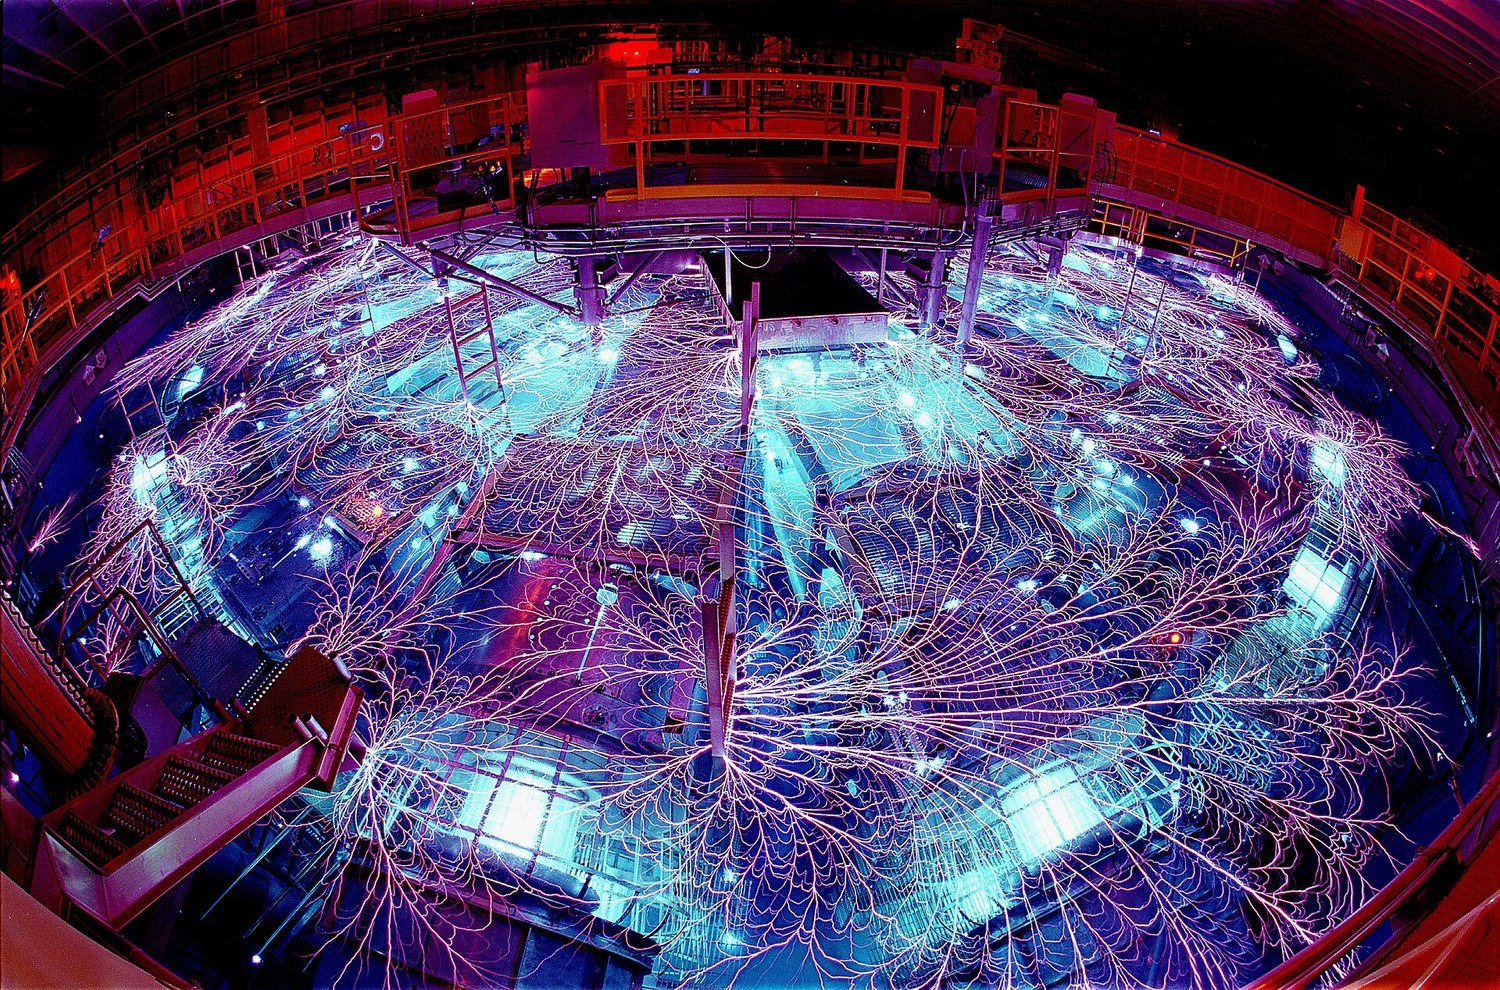
\includegraphics[width=0.72\textwidth]{../figures/aw_z_machine.jpg}
\caption{Z 装置：脉冲功率路线的高能量密度实验平台。本节算的冲击与烧蚀，在实验室里就是这台机器驱动出来的：电容器组把兆安级电流压进丝阵，把样品推到 Mbar 量级。}
\label{fig:photo-appaw2}
\figsource{ENERGY.GOV，Public domain（Wikimedia Commons）}
\end{figure}

\section{冲击与烧蚀：Rankine-Hugoniot 与 Mbar 量级}
\label{sec:app-aw-shock}

高能量密度实验最常用的「压」不是静压，而是冲击波。冲击波前后的三个守恒律
（质量、动量、能量）合称 Rankine-Hugoniot 关系。质量与动量守恒给出
\begin{equation}
\rho_0D=\rho_1(D-u_p),\qquad
P_1-P_0=\rho_0Du_p,
\label{eq:app-aw-rh1}
\end{equation}
其中 $D$ 是冲击速度、$u_p$ 是冲击后的粒子速度。取声明值 $D=50\ \mathrm{km\,s^{-1}}$、
$\rho_0=1000\ \mathrm{kg\,m^{-3}}$，并把能量守恒与状态方程合起来，
$\gamma=5/3$ 的强冲击压缩比有上限：
\begin{equation}
r\equiv\frac{\rho_1}{\rho_0}=\frac{\gamma+1}{\gamma-1}=4,
\qquad
u_p=\frac{D}{r}=12500\ \mathrm{m\,s^{-1}}.
\label{eq:app-aw-rh2}
\end{equation}
压缩比不是「想压多少压多少」，而是由 $\gamma$ 决定：$\gamma=5/3$ 最多四倍，
$\gamma\to1$（有电离、激发吸能）才可能更高。于是冲击压强
\begin{equation}
P=\rho_0Du_p=6.25\times10^{11}\ \mathrm{Pa}=6.25\ \mathrm{Mbar},
\label{eq:app-aw-rh3}
\end{equation}
离子温度由强冲击的能量分配给出
\begin{equation}
k_BT_i=\frac{2(\gamma-1)}{(\gamma+1)^2}m_iu_p^2=3.16216\times10^{-19}\ \mathrm{J}
=1.97366\ \mathrm{eV}.
\label{eq:app-aw-shockt}
\end{equation}
注意 $T_i$ 只有约 $2\ \mathrm{eV}$，而压强已经 $6.25\ \mathrm{Mbar}$——
这再次说明三个刻度彼此独立：冲击压缩可以在「不太热」的情况下把压强推到 Mbar。

激光直接驱动时，真正把靶推出去的是烧蚀压强。它不是 $I/c$，而是
火箭效应的产物：烧蚀掉的材料带着动量离开，反冲把剩余靶压紧。工程上常用标度律
\begin{equation}
P_\mathrm{abl}[\mathrm{Mbar}]
=8.6\,I_{14}^{2/3}\lambda_{\mu m}^{-2/3}
\ \Rightarrow\
P_\mathrm{abl}=45.3057\ \mathrm{Mbar}
=4.53057\times10^{12}\ \mathrm{Pa}=4530.57\ \mathrm{GPa},
\label{eq:app-aw-abl}
\end{equation}
其中 $I_{14}=I/10^{14}\ \mathrm{W\,cm^{-2}}$。与式~\eqref{eq:app-aw-prad} 的辐射压
$14.1569\ \mathrm{GPa}$ 相比高出 $320.026$ 倍，这个比值就是「为什么要烧蚀」的答案：
辐射直接推太弱，烧蚀把同样的通量放大两个半数量级。

\begin{table}[htbp]
\centering
\small
\caption{冲击与烧蚀（$D=50\ \mathrm{km\,s^{-1}}$、$\rho_0=1000\ \mathrm{kg\,m^{-3}}$、$\gamma=5/3$）}
\label{tab:app-aw-shock}
\begin{tabular}{p{4.4cm}p{4.2cm}p{4.2cm}}
\hline
量 & 值 & 口径 \\
\hline
强冲击压缩比 $r$ & $4$ & $(\gamma+1)/(\gamma-1)$ \\
粒子速度 $u_p$ & $12500\ \mathrm{m\,s^{-1}}$ & $D/r$ \\
冲击压强 $P$ & $6.25\ \mathrm{Mbar}$ & $\rho_0Du_p$ \\
冲击离子温度 $k_BT_i$ & $1.97366\ \mathrm{eV}$ & 强冲击能量分配 \\
烧蚀压强（标度律） & $45.3057\ \mathrm{Mbar}$ & $8.6(I_{14}\lambda_{\mu m}^{-2/3})^{2/3}$ \\
烧蚀压强/辐射压 & $320.026$ & 火箭效应放大倍数 \\
\hline
\end{tabular}
\end{table}

\begin{tip}{压缩比有上限，由 $\gamma$ 决定}{tip-app-aw-shock}
「把物质压到十倍密度」在 $\gamma=5/3$ 的强冲击里做不到：上限是四倍。
想更高只有两条路：让 $\gamma$ 靠近一（电离与激发把能量吃掉），
或者用非冲击的方式（准等熵压缩）。这也是惯性约束里「绝热与熵」那一节的关键。
\end{tip}

{\footnotesize
\textbf{出处：}Rankine-Hugoniot 关系与强冲击压缩比参照 Zel'dovich 与 Raizer 第 1 部分，
烧蚀压强标度律参照 Lindl《Inertial Confinement Fusion》与 Atzeni、Meyer-ter-Vehn 第 3 章。
标度系数 $8.6$ 是公开文献里的常用取值，本书把它明确标为声明输入。
}

\section{辐射温度与黑腔：温度是通量的四次方根}
\label{sec:app-aw-radiation}

间接驱动的核心是一个「把激光变成 X 射线」的盒子：黑腔。腔内壁吸收激光后升温、
再以 X 射线形式辐射，驱动靶丸。这里的物理只有一条：黑体辐射的温度由通量决定，
\begin{equation}
F_X=\eta_XI,\qquad
T_\mathrm{rad}=\left(\frac{F_X}{\sigma}\right)^{1/4},
\label{eq:app-aw-trad}
\end{equation}
其中 $\eta_X$ 是激光到 X 射线的转换效率（声明 $0.70$），
$\sigma$ 是斯特藩--玻尔兹曼常数。工况 N 的强度代入：
$F_X=2.97089\times10^{18}\ \mathrm{W\,m^{-2}}$，于是
\begin{equation}
T_\mathrm{rad}=\left(\frac{2.97089\times10^{18}}{5.670374\times10^{-8}}\right)^{1/4}
=2.69041\times10^{6}\ \mathrm{K}=231.842\ \mathrm{eV}.
\label{eq:app-aw-trad2}
\end{equation}
四次方根意味着温度对通量极不敏感：通量提高 $10\%$，温度只涨
$2.41137\%$。反过来，想把辐射温度从 $200\ \mathrm{eV}$ 提到 $300\ \mathrm{eV}$，
通量要涨 $(300/200)^4=5.06$ 倍：这是间接驱动激光器越造越大的根本原因。

对应的黑体能量密度与辐射压是
\begin{equation}
u_\mathrm{rad}=\frac{4\sigma T^4}{c}=3.96393\times10^{10}\ \mathrm{J\,m^{-3}},
\qquad
P_\mathrm{rad}=\frac{u_\mathrm{rad}}{3}=1.32131\times10^{10}\ \mathrm{Pa}
=0.132131\ \mathrm{Mbar}.
\label{eq:app-aw-urad}
\end{equation}
腔内壁并不是全吸收：反照率 $\alpha$（声明 $0.8$）把大部分辐射反射回去，
真正用来加热壁、进而再辐射的通量只有 $(1-\alpha)F_X$，于是有效驱动温度
\begin{equation}
T_\mathrm{wall}=\left(\frac{(1-\alpha)F_X}{\sigma}\right)^{1/4}
=1.79919\times10^{6}\ \mathrm{K}=155.042\ \mathrm{eV}.
\label{eq:app-aw-wall}
\end{equation}
$231.842\ \mathrm{eV}$ 是「假设全吸收」的上限，$155.042\ \mathrm{eV}$ 才是计入反照率后的
有效温度：两个数都要会算，前者是判据、后者是设计值。
入射的 $10.0\ \mathrm{kJ}$ 里，有 $7000\ \mathrm{J}$ 被转换成 X 射线，
其余留在激光与等离子体相互作用、散射与壁损耗里。

\begin{table}[htbp]
\centering
\small
\caption{黑腔的辐射温度账（$\eta_X=0.70$、反照率 $\alpha=0.80$、工况 N）}
\label{tab:app-aw-radiation}
\begin{tabular}{p{4.6cm}p{4.2cm}p{4.0cm}}
\hline
量 & 值 & 口径 \\
\hline
X 射线通量 & $2.97089\times10^{18}\ \mathrm{W\,m^{-2}}$ & $\eta_XI$ \\
辐射温度（全吸收） & $231.842\ \mathrm{eV}$ & $(F_X/\sigma)^{1/4}$ \\
黑体能量密度 & $3.96393\times10^{10}\ \mathrm{J\,m^{-3}}$ & $4\sigma T^4/c$ \\
黑体辐射压 & $0.132131\ \mathrm{Mbar}$ & $u_\mathrm{rad}/3$ \\
有效驱动温度 & $155.042\ \mathrm{eV}$ & 计入反照率 $0.8$ \\
X 射线能量 & $7000\ \mathrm{J}$ & $\eta_XE_L$ \\
通量 $+10\%$ 的温度响应 & $2.41137\%$ & 四次方根 \\
\hline
\end{tabular}
\end{table}

\begin{tip}{温度是通量的四次方根，不是能量的线性函数}{tip-app-aw-radiation}
「把激光能量翻倍，辐射温度会翻倍吗？」不会：温度按通量的 $1/4$ 次方走，
翻倍的通量只带来 $19\%$ 的温升。想让温度上一次台阶，必须同时动能量、
脉宽与光斑，或者干脆换更短的波长。
\end{tip}

{\footnotesize
\textbf{出处：}黑体辐射温度与反照率口径参照 Lindl 的间接驱动章节与
Atzeni、Meyer-ter-Vehn 第 3、8 章。
转换效率 $0.70$ 与反照率 $0.80$ 是公开文献的
常用量级，本书明确标为声明输入，不复制其黑腔几何与辐射流体结果。
}

\begin{figure}[htbp]
\centering
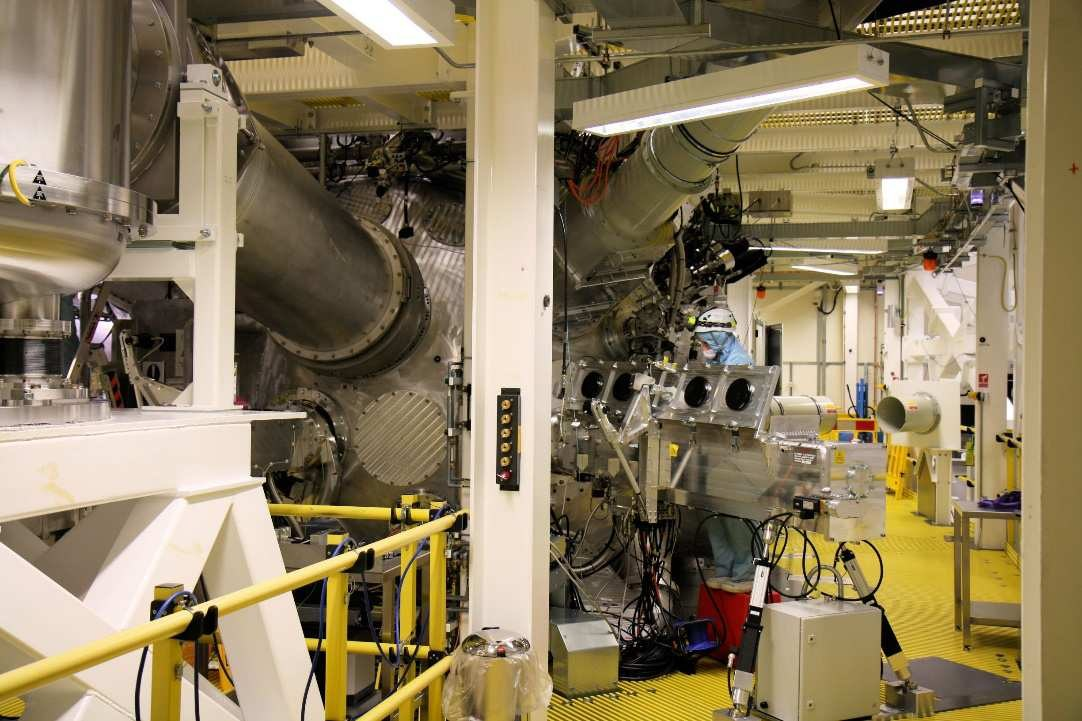
\includegraphics[width=0.78\textwidth]{../figures/aw_orion_chamber.jpg}
\caption{英国 Orion 激光装置的靶室：几束高功率激光同时打在一个毫米级靶上，在纳秒里造出只在恒星内部才有的压强与温度。实验室天体物理靠的就是这种「同无量纲数」的相似。}
\label{fig:photo-appaw3}
\figsource{Colin N. Danson 等，CC BY 4.0（Wikimedia Commons）}
\end{figure}

\section{实验室天体物理：无量纲相似}
\label{sec:app-aw-astro}

高能量密度物理还有一个身份：它是天体物理的「可重复实验版」。恒星内部、超新星遗迹、
吸积柱里的等离子体没法直接做实验，但如果两个系统的无量纲数相同，
流体方程的解就相似：这就是\textbf{标度律}（scaling law）的依据。
最常用的几个数是磁雷诺数、等离子体 $\beta$ 与欧拉数。声明一组实验室参数
（$\sigma=10^{6}\ \mathrm{S\,m^{-1}}$、$v=100\ \mathrm{km\,s^{-1}}$、
$L=1\ \mathrm{mm}$、$B=10\ \mathrm{T}$、$P=1\ \mathrm{Mbar}$）：
\begin{equation}
\mathrm{Rm}=\mu_0\sigma vL=125.664,
\qquad
\tau_\eta=\mu_0\sigma L^2=1.25664\times10^{-6}\ \mathrm{s}=1.25664\ \mathrm{\mu s}.
\label{eq:app-aw-rm}
\end{equation}
$\mathrm{Rm}\gg1$ 意味着磁场被流体「冻结」着带走（磁通量守恒），
$\mathrm{Rm}\ll1$ 意味着磁场扩散掉。实验室里 $\mathrm{Rm}\sim10^{2}$，
天体里可以到 $10^{10}$ 以上：要把实验室结果外推到天体，就得让 $\mathrm{Rm}$
尽量高，这通常靠提高速度与尺度，而不是提高电导率。

阿尔芬速度与等离子体 $\beta$ 是另外两个尺子：
\begin{equation}
v_A=\frac{B}{\sqrt{\mu_0\rho}}=282.095\ \mathrm{m\,s^{-1}},
\qquad
\beta=\frac{2\mu_0P}{B^2}=2513.27.
\label{eq:app-aw-va}
\end{equation}
$\beta\gg1$ 说明这是「高压低磁」的等离子体：磁场的动力学作用远小于热压，
与托卡马克芯部（$\beta$ 只有百分之几）正好相反。比较实验室与天体系统时，
必须同时对齐 $\mathrm{Rm}$、$\beta$ 与马赫数，只对齐其中一个会得到错的结论。
\begin{equation}
\frac{\mathrm{Rm}_\mathrm{astro}}{\mathrm{Rm}_\mathrm{lab}}
=79.5775\quad(\text{目标}\ \mathrm{Rm}=10^{4}),
\label{eq:app-aw-similarity}
\end{equation}
即要用 $1\ \mathrm{mm}$ 的实验室尺度去碰天体的磁冻结区，得把速度或尺度再抬两个量级——
这也是为什么这类实验往往用强激光驱动的高速流，而不是稳态装置。

\begin{table}[htbp]
\centering
\small
\caption{实验室与天体的无量纲数（声明：$\sigma=10^{6}\ \mathrm{S\,m^{-1}}$、$v=100\ \mathrm{km\,s^{-1}}$、$L=1\ \mathrm{mm}$）}
\label{tab:app-aw-astro}
\begin{tabular}{p{4.6cm}p{4.2cm}p{4.0cm}}
\hline
量 & 值 & 含义 \\
\hline
磁雷诺数 $\mathrm{Rm}$ & $125.664$ & 磁冻结判据 \\
磁扩散时间 $\tau_\eta$ & $1.25664\ \mathrm{\mu s}$ & $\mu_0\sigma L^2$ \\
阿尔芬速度 $v_A$ & $282.095\ \mathrm{m\,s^{-1}}$ & $B/\sqrt{\mu_0\rho}$ \\
等离子体 $\beta$ & $2513.27$ & 高压低磁 \\
要达到 $\mathrm{Rm}=10^{4}$ & 提高 $79.5775$ 倍 & 速度或尺度 \\
\hline
\end{tabular}
\end{table}

\begin{tip}{实验室天体物理靠的是无量纲数，不是「看起来像」}{tip-app-aw-astro}
两个等离子体「长得像」没有意义；只有 $\mathrm{Rm}$、$\beta$、马赫数这些无量纲数
对齐了，方程的解才相似。做这类实验前先把三个数算出来，比调激光参数更重要。
\end{tip}

{\footnotesize
\textbf{出处：}实验室天体物理的相似律与无量纲数选取参照 Remington、Drake、
Ryutov 的综述（\emph{Rev. Mod. Phys.} 78, 755 (2006) 等）以及
Drake 教材第 5 章。
本书只借判据与量级，不复制其靶设计与实验数据。
}

\section{估算练习}
\label{sec:app-aw-problems}

\textbf{练习 1} 一束 $\lambda=0.351\ \mathrm{\mu m}$ 的激光，强度
$I=10^{15}\ \mathrm{W\,cm^{-2}}$，求 $a_0$、$U_p$ 与 $v_\mathrm{osc}/c$。

\textbf{解答 1} 由式~\eqref{eq:app-aw-up}：
$a_0=\sqrt{10^{15}\times0.351^2/1.37\times10^{18}}=0.00948302$，
$U_p=\frac{1}{4}m_ec^2a_0^2=11.4882\ \mathrm{eV}=0.0114882\ \mathrm{keV}$，
$v_\mathrm{osc}/c=a_0/\sqrt{1+a_0^2}=0.0094826$。这个强度下电子完全是非相对论的，
强场效应（隧穿、相对论透明）都不会出现。

\textbf{练习 2} 若把电子密度提到 $10^{30}\ \mathrm{m^{-3}}$、温度降到 $5\ \mathrm{eV}$，
求费米能、简并参数与简并压。

\textbf{解答 2} $E_F=\frac{\hbar^2}{2m_e}(3\pi^2n_e)^{2/3}=36.4645\ \mathrm{eV}$，
$\Theta=5/36.4645=0.13712$（已进入简并区），
$P_\mathrm{deg}=\frac{2}{5}n_eE_F=2.3369\times10^{12}\ \mathrm{Pa}=23.369\ \mathrm{Mbar}$。
注意温度降了一半、密度升了十倍，冷压反过来超过热压——这就是 WDM 的两个修正此消彼长。

\textbf{练习 3} 冲击速度升到 $D=100\ \mathrm{km\,s^{-1}}$（其他条件同 AW.5），
求粒子速度、压强与离子温度。

\textbf{解答 3} 压缩比仍由 $\gamma$ 决定：$r=4$，
$u_p=D/r=25000\ \mathrm{m\,s^{-1}}$，
$P=\rho_0Du_p=25\ \mathrm{Mbar}$，
$k_BT_i=7.89466\ \mathrm{eV}$。速度翻倍 $\Rightarrow$ 压强翻四倍（$P\propto D^2$），
这在设计冲击实验时是很有用的一条。

\textbf{练习 4} 若激光到 X 射线的转换效率只有 $0.5$，而强度是
$10^{15}\ \mathrm{W\,cm^{-2}}$，求辐射温度。

\textbf{解答 4} $F_X=0.5\times10^{19}\ \mathrm{W\,m^{-2}}$，
$T_\mathrm{rad}=(F_X/\sigma)^{1/4}=264.066\ \mathrm{eV}$。
它比 AW.6 的 $231.842\ \mathrm{eV}$ 高，原因是这里的强度更高（$10^{15}$ 对
$4.24413\times10^{14}\ \mathrm{W\,cm^{-2}}$）——效率降了，通量仍更高。

\textbf{练习 5} 一束 $\lambda=0.8\ \mathrm{\mu m}$、$I=10^{19}\ \mathrm{W\,cm^{-2}}$
的激光，求 $a_0$、$U_p$ 与 Keldysh 参数（氢）。

\textbf{解答 5} $a_0=\sqrt{10^{19}\times0.8^2/1.37\times10^{18}}=2.16137$，
$U_p=\frac{1}{4}m_ec^2a_0^2=596.787\ \mathrm{keV}$，
$\gamma_K=\sqrt{13.6/(2\times596787)}=0.00337555$——深度隧穿区。
$a_0>1$ 说明电子已经是相对论的，与练习 1 形成鲜明对照。

\textbf{练习 6} 在 $L=1\ \mathrm{mm}$ 固定的情况下，要把 $\mathrm{Rm}$ 从
$125.664$ 提到 $10^{4}$，速度要提高多少倍？若速度不能提高，尺度要多大？

\textbf{解答 6} $\mathrm{Rm}\propto vL$，所以需要提高
$10^{4}/125.664=79.5775$ 倍。速度不能动时，尺度也要放大 $79.5775$ 倍，
即 $L=1\ \mathrm{mm}\times79.5775=79.5775\ \mathrm{mm}$——这已经超出激光驱动
实验的典型尺度，所以这类实验更愿意提高速度（用更强的驱动）。

\section{来源、分级与版权说明}
\label{sec:app-aw-source}

\begingroup\small
本附录的量级、判据与公式形式取自下列公开来源，按借鉴程度分级列出：

\begin{table}[htbp]
\centering
\small
\caption{本附录的借鉴来源}
\label{tab:app-aw-source}
\begin{tabular}{p{0.6cm}p{6.2cm}p{7.0cm}}
\hline
序号 & 来源 & 借用了什么 \\
\hline
1 & Drake, \emph{High-Energy-Density Physics}（Springer, 2006） & 三个刻度的框架；WDM 的定义与判据；实验室天体相似律 \\
2 & Atzeni \& Meyer-ter-Vehn, \emph{The Physics of Inertial Fusion}（Oxford, 2004） & 烧蚀压强标度律；黑腔辐射温度与反照率口径 \\
3 & Zel'dovich \& Raizer, \emph{Physics of Shock Waves and High-Temperature Hydrodynamic Phenomena}（1966/1967） & Rankine-Hugoniot 关系；强冲击压缩比与温度分配 \\
4 & Gibbon, \emph{Short Pulse Laser Interactions with Matter}（Imperial College Press, 2005） & $a_0$、$U_p$、Keldysh 参数与势垒抑制场 \\
5 & Lindl, \emph{Inertial Confinement Fusion}（Springer, 1998） & 间接驱动黑腔的能量账与转换效率量级 \\
6 & Ichimaru, \emph{Statistical Plasma Physics}（Addison-Wesley, 1992） & 强耦合判据（$\Gamma$、$N_D$）与等离子体参数口径 \\
7 & Remington, Drake, Ryutov 等，\emph{Rev. Mod. Phys.} 78, 755 (2006) 等综述 & 实验室天体物理的无量纲数选取与相似律表述 \\
\hline
\end{tabular}
\end{table}

\textbf{不复制声明：}本附录只借用上述来源的问题框架、判据形式与量级口径；
不复制其状态方程表、相图、靶设计图、实验数据、代码与习题。

\textbf{本附录没有涵盖什么：}完整的宽区状态方程模型（如 QEOS、SESAME 表的形式）、
辐射流体方程的数值解法（那属于附录 AC 的数值方法范畴）、
具体激光装置参数与靶设计、不透明度数据库，这几样这里都不展开。
需要做真实设计时，应当使用经过验证的状态方程表与辐射流体程序，
本附录的作用是把「该问哪几个问题、量级是多少」讲清楚。

\textbf{分级：}AW.1--AW.7 属于「读过本附录后能自己复算」的层级；
AW.5 的烧蚀标度律与 AW.7 的相似律属于「知道结论、会用量级」的层级；
$\mathrm{Rm}$ 与辐射流体耦合的细节属于进阶内容，正文只给判据。
\endgroup
